% 基本粒子
% 夸克|中微子|希格斯子|玻色子|光子|标准模型

\begin{issues}
\issueDraft
\end{issues}

\addTODO{图翻译成中文}
\begin{figure}[ht]
\centering
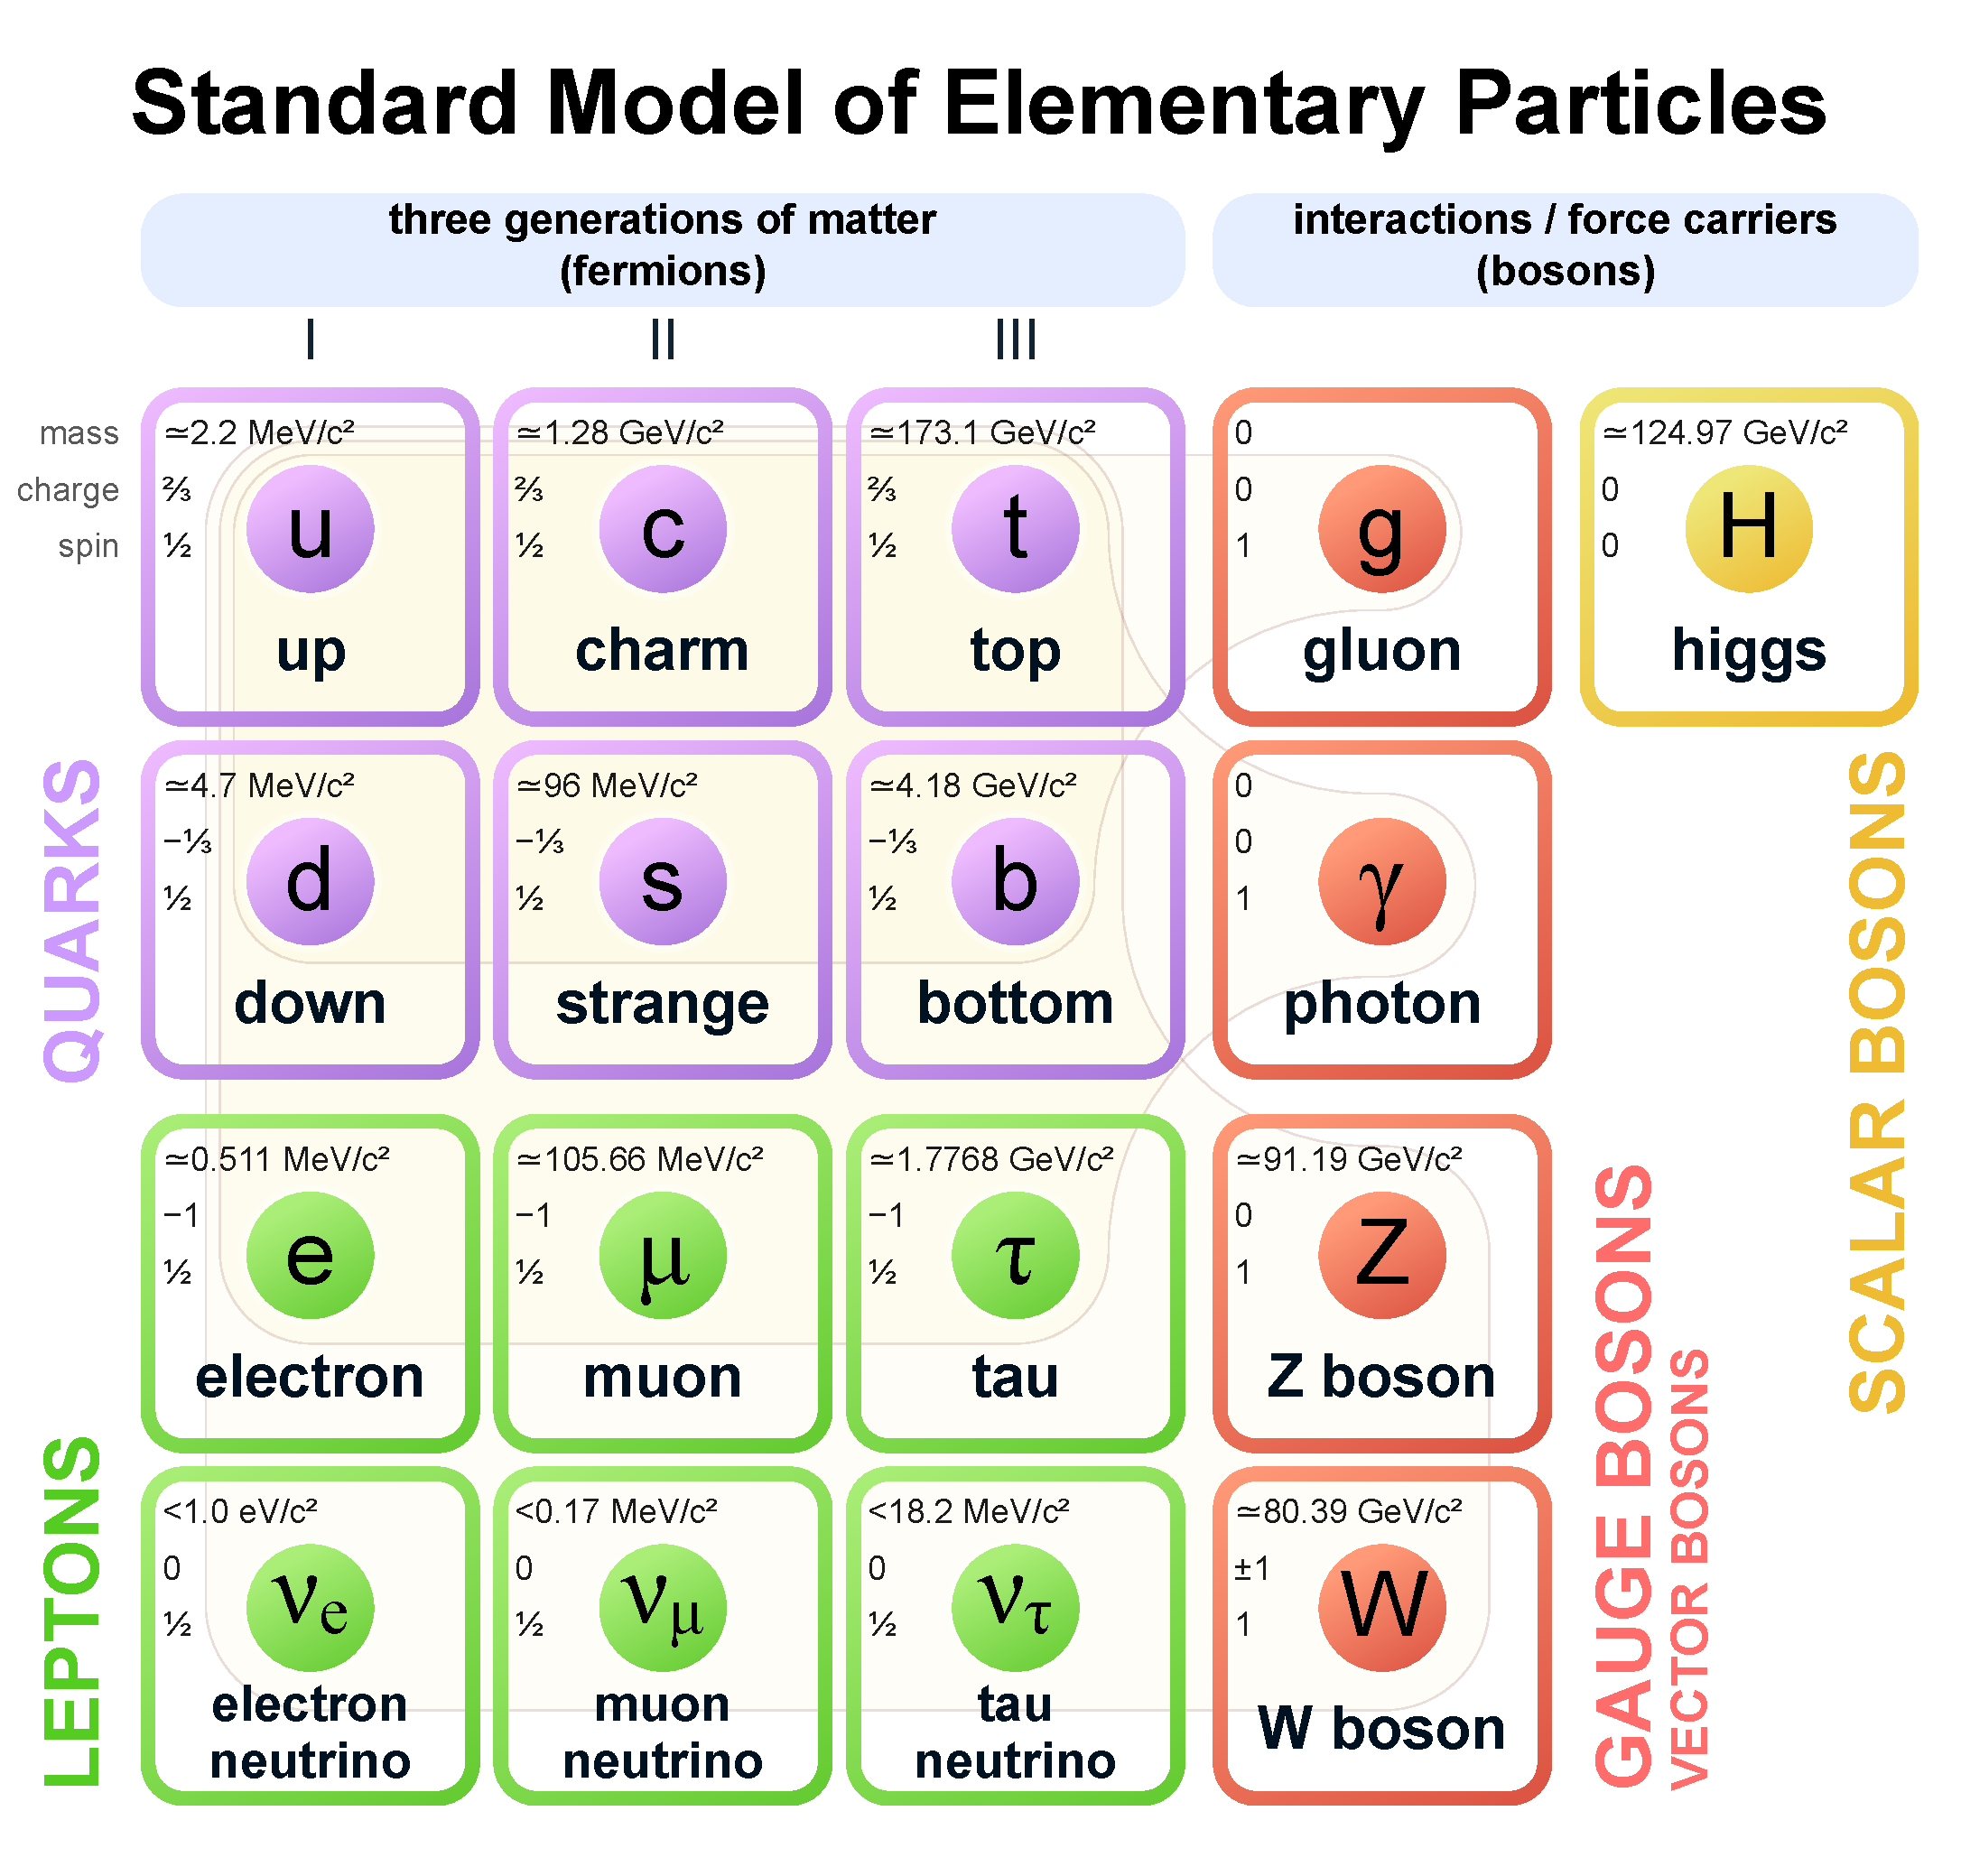
\includegraphics[width=12cm]{./figures/BasPar_1.pdf}
\caption{标准模型的基本粒子(来自维基百科)} \label{BasPar_fig1}
\end{figure}

费米子包括 6 种\textbf{夸克(quark)}和 6 种\textbf{轻子(lepton)}. 玻色子包括胶子, 光子, \textbf{Z 玻色子}和 \textbf{W 玻色子}, 以及\textbf{希格斯子(higgs)}.
